\section{MRT module}
\label{sec:mrt}

This section describes MRT module.

\subsection{MRT overview}
Multi-threaded Routing Toolkit (MRT) format was developed to encapsulate, export, and archive routing information in a standardized data representation.  The BGP routing protocol, in particular, has been the subject of extensive study and analysis which has been significantly aided by the availability of the MRT format. 

BGPmon MRT module gives an opportunity to receive data (updates and RIBs) from Routing Collectors (RC) such as University of Oregon Route Views Project\cite{routeviews}, RIPE NCC RIS Project\cite{riperis} and others.

MRT control module consists of a single MRT server thread and multiple MRT client threads.
\begin{itemize}
\item{\emph{MRT Server Thread:} It is a TCP server that listens on a specific port and spawns one thread for each client. }
\item{\emph{MRT Client Thread:} Each client thread receives data from a TCP connection.}
\end{itemize}

\subsection{MRT Server Thread}
The main data structure of MRT control module consists of the following fields:
\begin{itemize}
\item{\emph{listenAddr:} The listening socket of server thread binds to this address.  It is a string which could be a IPv4/IPv6 address or one of four keywords (ipv4loopback, ipv4any, ipv6loopback and ipv6any). After it is intialized from configuration, it could be set via command line interface (CLI) at runtime.}
\item{\emph{listenPort:} It is the port on which server thread listens.  It is an integer.  It also could be set via command line interface(CLI) at runtime after initialization.}
\item{\emph{enabled:} It indicates the status of server thread.  If it is false, server thread stops listening but the existing clients still run. Otherwise server thread listens on 'listenPort' and accepts allowed clients. It could be set via CLI after initialization.}
\item{\emph{maxMRTclients:} It is the max number of MRT clients. It could be set via CLI after initialization. }
\item{\emph{labeAction:} Its is the label action of MRT clients}
\item{\emph{activeMRTclients:} It is the number of connected MRT clients. }
\item{\emph{nextMRTclientID:} It is the ID for the next client to connect. }
\item{\emph{rebindFlag:} If listenAddr or listenPort changes, this flag will be set to TRUE. That means the listening socket of server thread will bind to the new address or port. It is set by CLI.  }
\item{\emph{shutdown:} It is a flag to indicate whether to stop the server thread. }
\item{\emph{lastAction:} It is a timestamp to indicate the last time the thread was active. }
\item{\emph{MRTListenerThread:} Reference to MRT thread. }
\item{\emph{firstNode:} First node in list of active MRT clients} 
\item{\emph{MRTLock:} It is a pthread mutex lock used to lock the MRT info linked list when MRT clients are added or deleted. }
\end{itemize}
This structure is mainly maintained by server thread. 

\subsection{MRT Client Thread}
MRT Client Thread has:
\begin{itemize}
\item{\emph{id:} Identification number of MRT client. }
\item{\emph{addr:} MRT Client's IP address. }
\item{\emph{port:}  MRT Clients's Port number. }
\item{\emph{socket:} MRT Client's socket for reading data }
\item{\emph{connectedTime:} MRT Client's connected time in seconds. } 
\item{\emph{lastAction:} MRT Client's last action timestamp.}
\item{\emph{qWriter:} This is a queue writer (see section \ref{sec:queue}). It is used to write messages to Peering queue. }
\item{\emph{deleteMRTClient:} Flag to indicate to close the MRT Client thread}
\item{\emph{labelAction:} Default label action. }
\item{\emph{next:}  Pointer to next MRT Client node. }
\item{\emph{MRTThreadID:}  Thread reference. }
\end{itemize}

\subsection{MRT Module Peering Design}

\subsubsection{Existing/3rd Party Routing Collectors}
Although BGPmon is able to peer directly with routers, there might be existing Routing Collectors in the Internet. BGPmon is able to work with these external RCs with a few modifications to the RC software. In order to provide correct routing data to the end user, RC should send both a RIB-IN tables and updates. Before describing changes to existing Routing Collectors, we should discuss software design of Routing Collector. Despite the fact that Routing Collector peers with other routers via TCP connection, it could provide routing data to BGPmon. In our design, we assume that Routing Collector can establish multiple TCP connections to BGPmon. Moreover, we need to answer the following questions: How Routing Collector should supply routing data to BGPmon and What is the right way to do that?
\begin{itemize}
	\item{\emph{For every peering router, Routing Collector establish a TCP session and forward routing data to BGPmon:} For example shown in Figure \ref{fig:routingcollector}, if Router 2 establishes BGP peering session with Routing Collector, RC creates a single TCP connection to BGPmon. For other routers, RC should create separate connections to BGPmon. This design makes peering session management easy: if BGP session between Router 2 and Routing Collector is failed, RC should close connection to BGPmon. }
	\item{\emph{Routing Collector establish only 2 TCP connections: one is update messages stream and second - RIB-IN messages stream:} Figure \ref{fig:routingcollector} shows example of the architecture. In our design, it does not matter how many peers RC has, RC will need only 2 TCP connections to BGPmon to send routing data from Routers 1-4. }
\end{itemize}



First answer looks reasonable because of peers up/down session management: for example, if Routing Collector's BGP peering failed with Router 2 and RC closes tcp connection to BGPmon, BGPmon must erase all BGP attributes and prefixes from its routing table associated with Router 2. But in our design we choose to use second approach. The main reason of this decision - number of connections (just two) required to send update and RIB-IN messages. Another important trade-off factor - insignificant code changes/additions to Routing Collector's software. These changes adds new functions to send routing data from Routing Collector to BGPmon. 


\begin{figure*}
\centering
\scalebox{0.55}{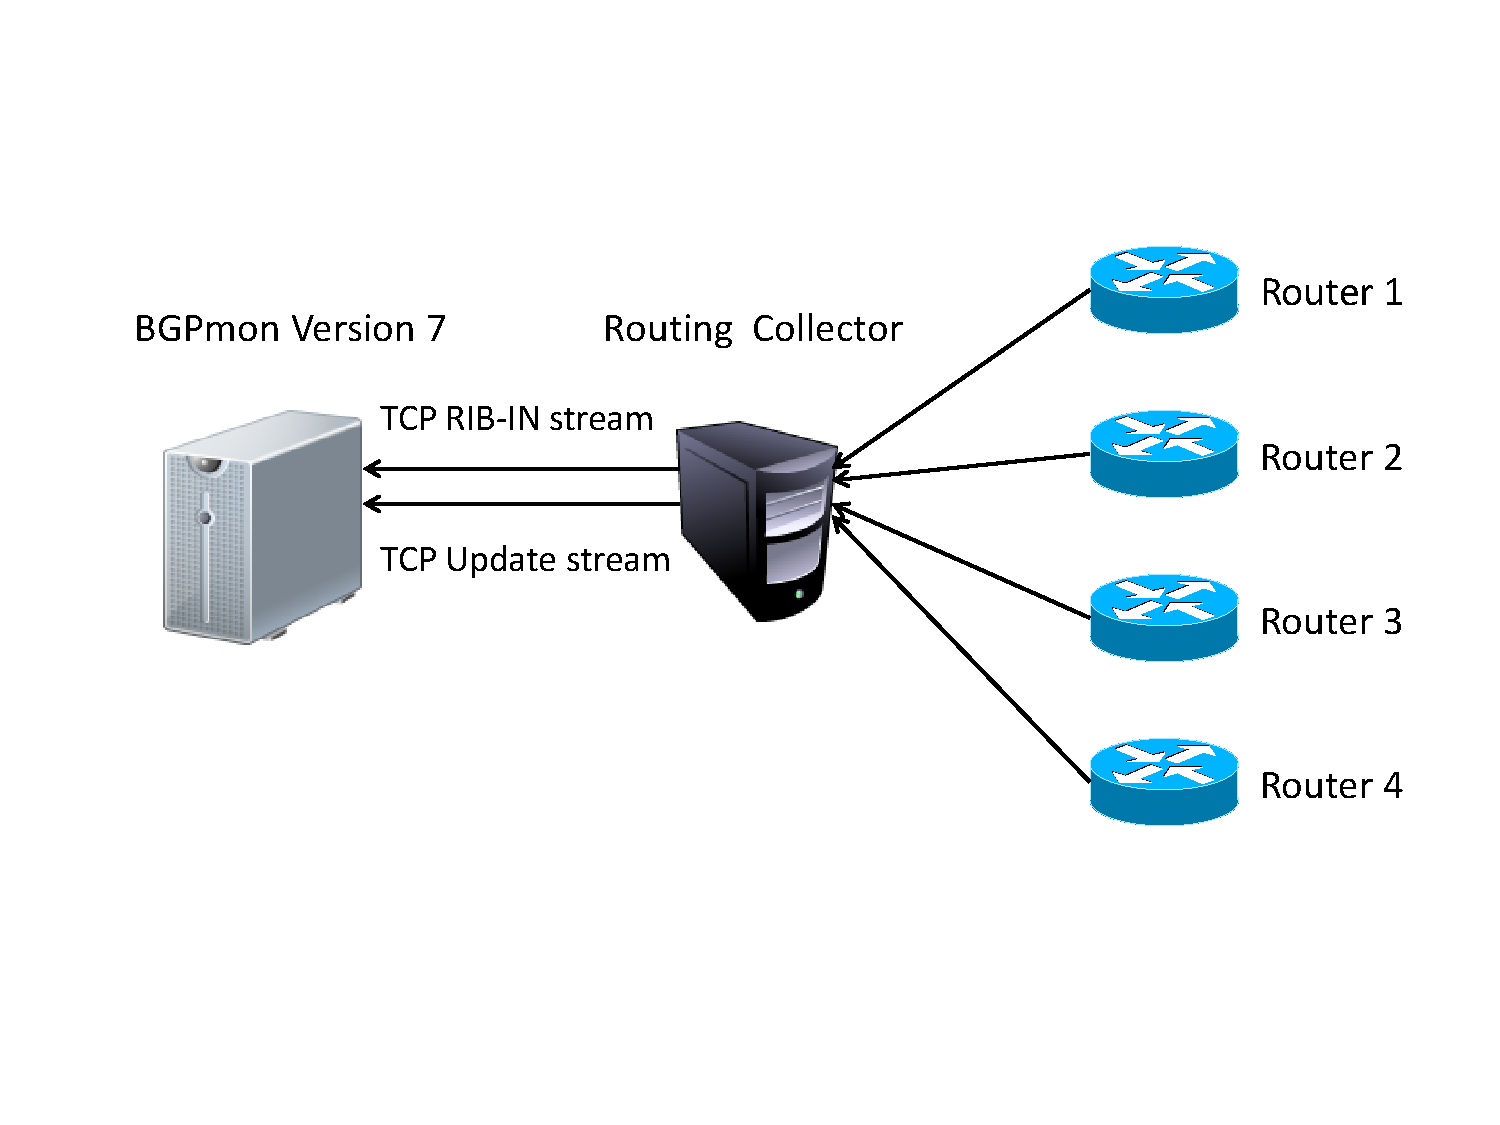
\includegraphics{figs/bgpmon-quagga.pdf}}
\caption{BGPmon and Routing Collector}
\label{fig:routingcollector}
\end{figure*}

In our design, we develop a patch to RC to support MRT format\cite{mrt}. Patch adds new functions to the Routing Collector to sends MRT messages (which contains updates or RIB-IN table) via TCP connection. Figure \ref{fig:routingcollector} shows example, where Routing Collector has multiple TCP sessions to Router 1-4 and just 2 TCP connections to BGPmon.  


% The Routing Collector has multiple BGP peering sessions with Routers 1-4. In our design, Routing Collector creates and uses multiple TCP connections to BGPmon. RC can create TCP session to send MRT update messages or to send MRT RIB-IN tables. This design was chosen because of MRT message format. Every header in MRT message contains each of router's IP address, port number and AS number. Using MRT header message, BGPmon can distinguish BGP messages originated from different RC's peers.

%in particular,   we are using this text to discuss our approach with a competing solution that could obsolete us.      critical to the discussion are the problems in integrating MRT streams.     what are the challenges in doing this?    what are the potential problems?   what is our design decision on the trade-offs.   more specificially
%I don't see a clear explanation of why the RC should send both a RIB table and updates.
%I don't see any example of how update streams and RIB tables are synchronized.

%I don't see any discussion of what happens if the RC sends a second BGP table for say router 1 in your figure.
%I don't see any discussion of why you should send several peers over single session or use one TCP connection for each peer.   for example,  do you send updates from Router 1, 2, 3, and 4 in one TCP session or four?  what are the trade-offs?

Every MRT message has a MRT header and body structure. The header for an update and RIB-IN messages has the same structure: a timestamp (time in seconds, when message originated), a type (type of MRT message), a subtype and a length (length of MRT message without the header). MRT body starts with peer's and RC's IP address, port number and AS number fields.  MRT body for update message contains BGP messages originated by peer, while the MRT body for RIB-IN message has the internal routing table generated by RC. Using MRT header message, BGPmon can distinguish BGP messages originated from different RC's peers.



% describe session structure
%In our implementation, Routing Collector maintains its peer sessions via TCP connection. If RC is using only 2 TCP streams to BGPmon to send routing data, it could create a peer up/down session management problem. For example, if TCP connection is lost to Router 1, RC should erase all BGP attributes and prefixes associated with Router 1. If peer reestablish connection, Routing Collector will create new session structure and start collecting routing data. Session management could be a tough problem for BGPmon - MRT message contains BGPmon is using MRT  message fields (peer IP address, port number and AS number fields) for maintaining "Session ID" structure described in section \ref{sec:peering}. The details of session management logic will be discussed in section \ref{sec:mrt:sessionmanagement}} and \ref{sec:mrt:sessionclosing}.

%describe possible oreder how updates or tables could be received and parsed
In our design, Routing Collector can create multiple TCP connections to BGPmon. Once the TCP connection is established, Routing Collector could send snapshot of MRT RIB-IN messages or MRT update messages. It's important to describe the order how update and table streams are synchronized in BGPmon:
\begin{itemize}
\item{What if first TCP stream contain MRT update messages and second TCP stream contain MRT RIB-IN messages?}
\item{What if first TCP stream contain RIB-IN messages and second TCP stream contain MRT update messages?} 
\end{itemize}

Answer for the first question is simple. For example, Routing Collector sends update message and then RIB-IN table message originated from Route 3. First, BGPmon receives update message and creates a new "Session" structure for Router 3. Then it gets a RIB-IN table for the Router 3. In our design, BGPmon extracts all BGP attributes and prefixes from RIB-IN message and store them in internal BGPmon routing table linked with Router 3 "Session" structure.

Answer for the second question is different: assume that BGPmon receives a RIB-IN table from Router 3 first and update message later. BGPmon will create a new session structure for Router 3 and copy all RIB-IN tables to internal routing table. Future update messages will add or withdraw routes in BGPmon table. 


%BGPmon will store all MRT RIB-IN message in queue buffer. Then, for each of update message, which contain Router 3 IP address, port number and AS number, MRT module will search in queue buffer for same values.
%Second question described correct order of receiving message. Ideally, 

%MRT module will store MRT RIB-IN message in queue buffer. Then, for each of update message, which contain Peer IP address, port number and AS number, MRT module will search in queue buffer for same values. If these values are found in queue buffer, MRT module will extract BGP attributes and prefixes from buffer, create new BMF messages and send them to PeerQueue. Then MRT module will convert update message to BGPmon's internal BMF format and apply this message to PeerQueue. Overall, second question describes the ideal behavior of Routing Collector: first of all, its necessary to send correct picture of routing data (RIB-IN messages). Then Routing Collector should periodically send MRT update messages to change (add or withdraw) BGPmon's internal RIB-IN table.

Also, it's important to mention another issue in this design: What about synchronization of these 2 streams? What should be a time period (timer) between two connections? And can 2 streams overlap? Answer for the last question is yes, they can. To prevent overlapping, BGPmon tracks what stream is processing. If BGPmon processing RIB-IN stream, it will buffer all further update messages and apply them after table extracting is done. Also, is case if BGPmon receiving update stream first and if time period between two connections is too long, we could damage already created BGPmon's routing table. In another case, if time period is too small, two connections could overlap and create a routing mess. In our design, we accept the fact that 5 to 10 minutes period is optimal to use between two streams and this value won't change BGPmon's routing table dramatically.


%I don't see any discussion of how you close a session for a particular session.   for example,   how do you close the session to only router 3.
%I don't see any discussion of what happens if the connection between the  router and the RC fails.    for example,  what happens if RC to router 2 connection fails then restarts.
Another significant design issue is TCP session failure between RC and its peers. For example, BGP peering session between RC and Router 2 fails or closes. Once the session is down,  BGPmon no longer receives updates to the table and the table stored in BGPmon can quickly become out of date.  BGPmon should detect the peering session is now down and delete the routing table for Router 2. For directly connected peers, BGPmon immediately detects the peering session failure following the procedure set out in the BGP standard \cite{bgprfc}. For an indirectly connected peer such as Router 2 in Figure \ref{fig:routingcollector}, the Route Collector has learned the peer is down but this information should be sent to BGPmon. 
% signal part
In order to do that correctly, RC should send a signal to BGPmon that session to Router 2 is failed. Without an explicit signal from the Route Collector, it is difficult for BGPmon to infer that the session failed.
% If RC won't send a signal to BGPmon, Router 2 routing table in BGPmon can become out of date. 
Instead of trying to infer when a session has failed,  the Routing Collector must send an explicit signal indicating the session to Router 2 has failed. In our design, this signal is a MRT RIB-IN message. Header of this message has a Router 2 peering IP address, port and AS number, while message body is empty. When BGPmon receives this message, it should erase all BGP attributes and prefixes associated with Router 2 session structure.
In case, when signal message is lost or did not occur, there might be two problems:
\begin{itemize}
\item{\emph{BGPmon lost a TCP session to Routing Collector:} BGPmon should delete all tables associated with RC peers.}
\item{\emph{Route Collector did not send a signal or signal was incorrect:} It could be a complex problem for BGPmon to keep all routing data in current state. If Route 2 connection to RC failed, RC won't be able to send BGPmon any update message.}
\end{itemize}

The important design issue here is how to manage data from peer which reestablished connection with Routing Collector. For example, Routing Collecter restarts BGP session with Router 4, BGPmon will start receiving routing data from RC. First of all RC should provide a RIB-IN table from Router 4. It couldn't be done immediately after tcp connection is opened. Routing Collector needs to create its own RIB-IN table. After that, RC must send table to BGPmon. Secondly, all BGP update message originated from Router 4 should be send to BGPmon after the first step is done. 

In our design, as described previously, BGPmon is able to receive RIB-IN table multiple times from the same Router 4. It could happen when TCP connection between RC and Router 4 fails and restarts again.  In order to have correct routing picture in BGPmon, we assume that every time when BGPmon receives RIB-IN table, it should erase all BGP attributes and prefixes associated with "Session" structure (in our example, Router 4 "Session" structure) from its table and apply the new table by extracting data from MRT RIB-IN message. 

Moreover, we should discuss another important issue is how Routing Collector manage BGP peers with different AS number (ASN) lengths in BGP attributes\cite{bgprfc}. Also, we will discuss problems which could occur and trade-offs in our design. Following the topology example shown in Figure \ref{fig:routingcollector}, lets assume that Router 1 and Router 2 are using 2-byte ASNs, while Router 3 and 4 - 4-byte ASNs. When Routing Collector establishes BGP peering session with the Routers, each of Routers will send BGP capabilities to indicate what AS length they support. In particular example, Routers 1,2 will send BGP capabilities that both of them support 2-byte ASN length and Router 3,4 - 4-byte ASN length. In this case, Routing Collector should organize routing table properly for each of the peers. There could be two possible solutions how to handle peers with different ASN lengths:
\begin{itemize}
\item{Routing Collector could maintain a routing table with different AS number lengths for each of peers.}
\item{Routing Collector could use 4-byte AS number length as default for all peers.}
\end{itemize}

Fist solution looks reasonable - Routing Collector need to have key parameter, which will store AS number length value for each of peering Routers. This assumption makes routing table not perfectly organized, for each of peers, there will be different AS path length and different peer session structure. In terms of future Internet development and simplicity of adding new features to the routing protocols, we think that Routing Collector should use a 4-byte AS number length as default: RC should not worry about peer AS number length. It could use 4-byte length fields to store 2-byte or 4-byte long AS numbers. 

If Routing Collector is using 4-byte ASN length a default ASN length for all of peers, it creates other problems for BGPmon: Routing Collector could send routing table to BGPmon in 4 byte AS number length format, while update messages from peers could be 2-byte long. In example shown in Figure \ref{fig:routingcollector}, Routing Collector could send RIB-IN tables from Router 1, which is using 2-byte AS length, in 4-byte format. Moreover, Routing Collector will provide further update message in 2-byte format from Router 2. This problem might create a mess in BGPmon's routing table. In order to eliminate following issues, we made few important changes to our design: 
\begin{itemize}
\item{\emph{If, Routing Collector sends RIB-IN table in 4-byte format from Router 1 and further update messages from the same routers are 2-byte long, BGPmon should convert Router 2's entire routing table to use 2-byte ASN length.}} 
\item{\emph{If, Routing Collector sends RIB-IN table in 4-byte format from Router 1 and further update messages from the same routers are 4-byte long, BGPmon won't add any changes to its routing table. }} 
\item{\emph{If, Routing Collector sends RIB-IN table in 2-byte format from Router 1 and further update messages from the same routers are 2-byte long, BGPmon won't add any changes to its routing table.}}
\item{\emph{If, Routing Collector sends RIB-IN table in 2-byte format from Router 1 and further update messages from the same routers are 4-byte long, BGPmon print a error to log.}}
\end{itemize}











% Route Collector should send an empty RIB-IN message for Router 2. If connection between Router 2 and Route Collector restarts, RC should send 

% For example, if TCP connection is lost between Router 3 and RC. In our design, RC will send empty RIB-IN tale only for Router 3 
%Routing Collector maintains TCP session with its peers and MRT message format does not allow us to know, when TCP connection fails or closes between Routing Collector and peer. In our design, instead of adding and keep tracking timeout value for each of created "SessionID's", 

%If TCP connection between the Router 2 and the RC fails, RC sends RIB-IN message with empty routing table of Router 2. At BGPmon side, MRT module will erase all BGP attributes and prefixes associated with this peer. If Routing Collector restarts connection with a Router 2, it sends newly created MRT RIB-IN and update messages to BGPmon. Further, MRT module will create new "Session" structure with BGP attributes and prefixes. 

%If TCP connection restarts, RC will recreate its own routing table and send 

%ample,  what happens if RC to router 2 connection fails then restarts.

%In case if Routing Collectors sends entire MRT RIB-IN messages periodically, BGPmon MRT module will reset all routing tables of "SessionID's" associated with Routing Collector's data and create new "Session" structures.

 
%We added a timeout value for each of created sessionID's. If no MRT update message arrived during the timeout period, %we assume that TCP session fails and Session Close function should be called. If Routing Collector reestablish %connection with its peer, new MRT RIB-IN and update message should be forwarded to BGPmon.

%describe possible situations with number of tcp connections: 



%Routing Collector sends MRT data in different ways: 

%It's important to mention about the order of receiving update and RIB-IN messages: first, MRT module receives RIB-IN message snapshot from RC and then update %messages only to add or withdraw routing changes to BGPmon's internal RIB-IN routing database. Future RC RIB-IN messages should be discarded.
\subsubsection{BGPmon MRT module overview}
BGPmon MRT module supports 2 types of MRT messages (see \cite{mrt}):
\begin{itemize}
\item{\emph{Update message:} This message has a header structure with "BGP4MP" type and "BGP4MP\_MESSAGE" or "BGP4MP\_MESSAGE\_ AS4" subtype and message body with  BGP attributes and prefixes. }
\item{\emph{RIB-IN message:} This messages has header structure with "TABLE\_DUMP\_V2" type and contains all routing data from Routing Collector (RC).}
\end{itemize}

Messages with other MRT header types (for example OSPF, ISIS) are ignored and error message will appear in log file or stdio output.



\subsubsection{Processing MRT updates}
MRT update message, received from Routing Collector, has following fields:
\begin{itemize}
\item{\emph {Peer address:} Peer IPv4 or IPv6 address}
\item{\emph {Local address:} RC IPv4 or IPv6 address}
\item{\emph {Peer AS:} Peer AS number, could be 2-bytes or 4-bytes length}
\item{\emph {Local AS:} RC AS number, could be 2-bytes or 4-bytes length}
\item{\emph {BGP Message:} BGP Message with attributes and prefixes}
\end{itemize}
MRT module parses update message following MRT draft specification and converts it to internal BMF BGPmon message. Then new BMF message applied to PeerQueue.

\subsubsection{Processing MRT RIB-IN tables}
Routing Collector sends RIB-IN table message only once after successful TCP connection. RIB-IN messages have MRT header structure with "TABLE\_DUMP\_V2" type and current timestamp. Main body message contains list of all peer clients connected to Routing Collector and their BGP attributes and prefixes. BGPmon MRT module parses this message, creates and sends new BMF message to PeerQueue.

\subsubsection{Session Management}
\label{sec:mrt:sessionmanagement}
When Routing Collector establishes TCP connection to BGPmon and new messages (update or RIB-IN table) arrives, MRT module makes the following checks based on first arrived message:
\begin{itemize}
\item{\emph{First message is RIB-IN message:} MRT module creates RIB-IN queue buffer and copy all RIB-IN messages to the buffer.}
\item{\emph{First message is update message:} MRT module creates new Session structure with sessionID (based on Peer IP address, port and AS number), searches through the RIB-IN queue buffer for BGP attributes and prefixes associated with sessionID. Then MRT module creates new BMF messages and sends them to PeerQueue. }
\end{itemize}

\subsubsection{Session Closing}
\label{sec:mrt:sessionclosing}
RC's TCP connection sends multiple update messages from its peers, MRT module keeps track of all SessionIDs created with particular RC. If RC's connection fails or closes, MRT module will:
\begin{itemize}
\item{{Change Label Action:} Change all states of previously created Session IDs to "stateError". }
\item{{Delete Attributes:} Delete all BGP attributes and prefixes from BGPmon internal RIB-IN table. }
\end{itemize}

\subsubsection{2 bytes and 4 bytes AS length format}
BGPmon MRT module supports update and RIB-IN messages containing 2-bytes or 4-bytes length AS Path. Current software implementation of Routing Collectors could send updates or RIB-IN messages using different format. Based on received data, MRT module makes following changes to ASPath associated with SessionID structure:
\begin{itemize}
\item{\emph{First message is RIB-IN and has 2 byte ASN}}
	\begin{itemize}
		\item{\emph{Second message is update and has 2 bytes ASN:} MRT module will process this update message without any changes}
		\item{\emph{Second message is update and has 4 bytes ASN:} MRT module will print a error and wont process this message}
	\end{itemize}
\item{\emph{First message is RIB-IN and has 4 bytes ASN}}
	\begin{itemize}
		\item{\emph{Second message is update and has 2 bytes ASN:} MRT module will convert internal BGPmon routing table to 2 byte ASPath length}
		\item{\emph{Second message is update and has 4 bytes ASN:} MRT module will process this update message without any changes}
	\end{itemize}
\item{\emph{First message is update and has 2 bytes ASN}}
	\begin{itemize}
		\item{\emph{Second message is RIB-IN and has 2 bytes ASN:} MRT module will process this update message without any changes}
		\item{\emph{Second message is RIB-IN and has 4 bytes ASN:} MRT module will convert ASpath of RIB-IN message to 2 byte ASN }
	\end{itemize}		
\item{\emph{First message is update and has 4 bytes ASN}}
	\begin{itemize}
		\item{\emph{Second message is RIB-IN and has 2 bytes ASN:} MRT module will print error and wont process this message}
		\item{\emph{Second message is RIB-IN and has 4 bytes ASN:} MRT module will process this update message without any changes}
	\end{itemize}	
\end{itemize}

\subsubsection{Corrupted MRT messages}


The MRT module in BGPmon reads fixed-size data chunks from the socket connection and expects well-formatted MRT messages. However, the Routing Collector may send  MRT messages out of order and thus corrupt the internal data structures in BGPmon. To this end, MRT module attempts to recover from corrupted MRT messages.  

\note{BGPmon MRT module is able to recover from corrupted MRT update messages only. Currently there is no recover solution for MRT RIB-IN table messages.
}




The important design decision here is how MRT module finds the next valid MRT update message. The MRT module include two-step procedure for MRT update messages: detection of corrupted messages and recovering from corruption. 

To detect corrupted MRT update message, MRT module validates MRT common header. This procedure includes MRT header values tests. 
\begin{itemize}
\item{MRT module validates the MRT header timestamp. MRT module checks if MRT timestamp value is not bigger than the current timestamp. }
\item{MRT module validates the MRT type and subtype values according to MRT RFC \cite{mrt}. MRT module checks for \emph{TABLE\_DUMP\_V2} and \emph{BGP4MP} types and all inclusive subtypes.}
\item{MRT module validates the MRT header length. In particular, it checks that the MRT message length is not bigger than the max MRT update message (that depends on corresponding MRT type and subtype). }
\end{itemize}

If one of validation tests fail, MRT module start recovering from corrupted MRT update message. This procedure includes following:

\begin{itemize}
\item{Since every MRT update message include BGP message from the wire, the MRT module will try to find valid BGP marker value: 16 bytes of data that contains "0xFF" values. The MRT module reads byte by byte from the socket connection until it finds the BGP marker. }
\item{Once the BGP marker is found, MRT module will try to read 2 bytes of length. However, its important to verify that previous 16 bytes are valid BGP marker. To this end, the MRT module reads one byte of BGP length and checks if the byte value is  not equal to "0xFF" marker value. Upon failure, MRT module continues to read byte by byte from the socket to get the valid BGP message length. Upon success, MRT module will read the second byte of BGP length and merge two bytes together to get the value of BGP message length. }
\item{Lastly, MRT module uses BGP message length to read the remaining number of bytes to get to the end of the BGP message.}
\item{At this point, MRT module expects the start of new MRT update message.}
\end{itemize}



\subsection{Design Philosophy}
The important design decision here is that BGPmon MRT module can receive data from any kind of Routing Collector which supports MRT format specification. For example routing software such as Zebra or Quagga needs a small patch to support MRT format. This patch is available in BGPmon distribution. 



In the design of MRT module, one of important issues is how to handle order of update or RIB-IN messages with 2 or 4 bytes AS Path length. Today's peering routers rarely use 4-bytes AS Path length and they trying to avoid problem with 4 to 2 bytes ASPath conversion. MRT module is using simple solution described in previous subsection.

